\subsection{Introduction}
\paragraph{Idea} Sparse dictionary learning is a representation learning method which aims at finding a sparse representation of the input data (in form of a linear combination of basic elements (called Atoms). The idea of using a learned dictionary instead of a predefined one is based on wavelets. The sparse learned models has recently led to state-of-the-art result for denoising, classification,...
%UNSPERVISED LEARNING=========================================================+
\paragraph{Unsupervised learning} Only use the inputs $x^{(t)}$ ( $X = [x_1,....,x_n]$ in $\R^{m \times n}$) for learning. Automatically extract meaningful features of our data, leverage the availability of unlabeled data and add a data-dependent regularize to trainings.\\

Sparse coding is one of the methods used for unsupervised learning  (like restricted Boltzmann machines and autoencoders).\\
The idea behind sparse coding is: For each $x^{t}$ find a latent representation $\alpha^{t}$ such that:
\begin{itemize}
 \item[$\bullet$] It is sparse: the vector $\alpha^{t}$ has many zeros (only few nonzero elements)
 \item[$\bullet$] We can reconstruct the original input $x^{(t)}$ as well as possible.
\end{itemize}
That mean, more formally:\\

%Formulation du problème=============================
\begin{center}
 $\min\limits_{D} \frac{1}{T} \sum_{t=1}^{T}  \min\limits_{\alpha^{(t)}} \frac{1}{2} \| x^{(t)} - D \hspace{3px} \alpha^{(t)} \|_2^2 + \lambda \|\alpha^{(t)} \|_1$\\
\end{center}

 %Explicaiton de la formulation=========================
 \begin{itemize}
 \item[$\bullet$] D is a matrix of weights, usually refer to that matrix as a dictionary matrix (containt atoms) with $D \in  \R^{m \times k}$ ( k the number of atoms)
  \item[$\bullet$] $\| x^{(t)} - D \hspace{3px} \alpha^{(t)} \|_2^2 $ is the reconstruction error
  \item[$\bullet$]$ D \hspace{3px} \alpha^{(t)}$ is the reconstruction of $\hat{x}^{(t)}$
  \item[$\bullet$]$\|\alpha^{(t)} \|_1$ is the sparsity penalty (more 0 in h we have, better it is)
 \end{itemize}
This two objectives fight each other. But it still a optimization problem (cf min), and we'll try to optimize it for each training example $x^{(t)}$. This is why we have a sum over all the training examples.
\newline

%Contraintes sur D======================================
\indent We also constrain the columns of D to be of norm 1 (otherwise, D could grow big while $\alpha^{(t)}$ becomes small to satisfy the prior). And sometimes the columns are constrained to be no greather than 1.\\

However, $\alpha^{(t)}$ is now a complicated function of $x^{(t)}$:\\
Encoder is the minimization $\alpha(x^{(t)}) = arg\min\limits_{\alpha^{(t)}}= \frac{1}{2} \| x^{(t)} - D \hspace{3px} \alpha^{(t)} \|_2^2 + \lambda \|\alpha^{(t)} \|_1$, so the optimization problem is more complicated than a simple non linear problem.\\
The idea to solve this minimization problem is \cite{NIPS2006_2979}

\begin{lstlisting}[language=Python,frame=single]
while D not_converged :
    Fix D
    Minimize alpha     (1) // Sparse Coding step
    Fix alpha
    Minimize D           (2) // Update Dictionary step
\end{lstlisting}

But there are some improvement like K-SVD algorithm \cite{KSVD}, which compute column by column a SVD computation over the relevant examples.
%DICTIONARY==================================================================+  
\paragraph{Dictionary}
We can also write $\hat{x}^{(t)} = D\hspace{3px} \alpha(x^{(t)}) \displaystyle\sum_{\substack{k s.t.\\ \alpha(x^{(t)})_k\neq 0}}  D.,_k \alpha(x^{(t)} )_k$
\begin{figure}[h]
 \centering
 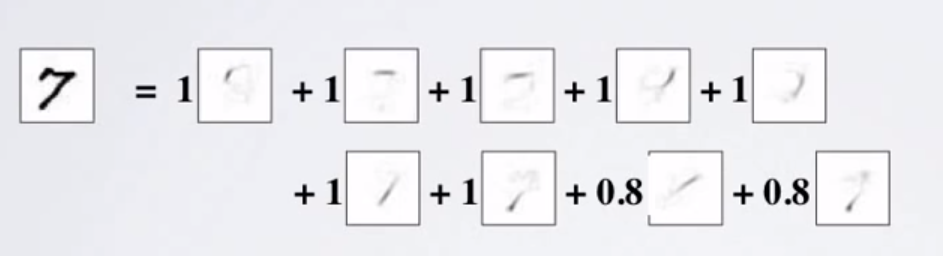
\includegraphics[scale=0.5]{spacecoding_1.png}
 % spacecoding_1.png: 943x256 px, 96dpi, 24.95x6.77 cm, bb=0 0 707 192
  \caption{Example of reconstruction using sparse coding}
\end{figure}

The images refer to $D.,_k$ (columns of D wich are not equals to 0) and the factor (1 or 0.8 in this case) refer to $\alpha(x^{(t)} )_k$
\\We also refer to D as the dictionary:
\begin{itemize}
 \item[$\bullet$]in certain applications, we know what dictionary matrix to use
 \item[$\bullet$]often however, we have to learn it
\end{itemize}

In general we have $k<<n$ . But we can use an overcomplete dictionary with $k > m$.
